% Options for packages loaded elsewhere
\PassOptionsToPackage{unicode}{hyperref}
\PassOptionsToPackage{hyphens}{url}
\PassOptionsToPackage{dvipsnames,svgnames,x11names}{xcolor}
\documentclass[
  11pt,
]{article}
\usepackage{xcolor}
\usepackage[margin=1in]{geometry}
\usepackage{amsmath,amssymb}
\setcounter{secnumdepth}{5}
\usepackage{iftex}
\ifPDFTeX
  \usepackage[T1]{fontenc}
  \usepackage[utf8]{inputenc}
  \usepackage{textcomp} % provide euro and other symbols
\else % if luatex or xetex
  \usepackage{unicode-math} % this also loads fontspec
  \defaultfontfeatures{Scale=MatchLowercase}
  \defaultfontfeatures[\rmfamily]{Ligatures=TeX,Scale=1}
\fi
\usepackage{lmodern}
\ifPDFTeX\else
  % xetex/luatex font selection
\fi
% Use upquote if available, for straight quotes in verbatim environments
\IfFileExists{upquote.sty}{\usepackage{upquote}}{}
\IfFileExists{microtype.sty}{% use microtype if available
  \usepackage[]{microtype}
  \UseMicrotypeSet[protrusion]{basicmath} % disable protrusion for tt fonts
}{}
\makeatletter
\@ifundefined{KOMAClassName}{% if non-KOMA class
  \IfFileExists{parskip.sty}{%
    \usepackage{parskip}
  }{% else
    \setlength{\parindent}{0pt}
    \setlength{\parskip}{6pt plus 2pt minus 1pt}}
}{% if KOMA class
  \KOMAoptions{parskip=half}}
\makeatother
\usepackage{longtable,booktabs,array}
\newcounter{none} % for unnumbered tables
\usepackage{calc} % for calculating minipage widths
% Correct order of tables after \paragraph or \subparagraph
\usepackage{etoolbox}
\makeatletter
\patchcmd\longtable{\par}{\if@noskipsec\mbox{}\fi\par}{}{}
\makeatother
% Allow footnotes in longtable head/foot
\IfFileExists{footnotehyper.sty}{\usepackage{footnotehyper}}{\usepackage{footnote}}
\makesavenoteenv{longtable}
\usepackage{graphicx}
\makeatletter
\newsavebox\pandoc@box
\newcommand*\pandocbounded[1]{% scales image to fit in text height/width
  \sbox\pandoc@box{#1}%
  \Gscale@div\@tempa{\textheight}{\dimexpr\ht\pandoc@box+\dp\pandoc@box\relax}%
  \Gscale@div\@tempb{\linewidth}{\wd\pandoc@box}%
  \ifdim\@tempb\p@<\@tempa\p@\let\@tempa\@tempb\fi% select the smaller of both
  \ifdim\@tempa\p@<\p@\scalebox{\@tempa}{\usebox\pandoc@box}%
  \else\usebox{\pandoc@box}%
  \fi%
}
% Set default figure placement to htbp
\def\fps@figure{htbp}
\makeatother
\setlength{\emergencystretch}{3em} % prevent overfull lines
\providecommand{\tightlist}{%
  \setlength{\itemsep}{0pt}\setlength{\parskip}{0pt}}
\usepackage{bookmark}
\IfFileExists{xurl.sty}{\usepackage{xurl}}{} % add URL line breaks if available
\urlstyle{same}
\hypersetup{
  pdftitle={Metric autopsy: a metric-agnostic gate system for separating biological signal from QC and technical artifacts in single-cell metrics},
  pdfauthor={Theodor Spiro},
  colorlinks=true,
  linkcolor={RoyalBlue},
  filecolor={Maroon},
  citecolor={Blue},
  urlcolor={RoyalBlue},
  pdfcreator={LaTeX via pandoc}}

\title{Metric autopsy: a metric-agnostic gate system for separating
biological signal from QC and technical artifacts in single-cell
metrics}
\author{Theodor
Spiro\thanks{Vaika Inc.\quad ORCID 0009-0004-5382-9346\quad \texttt{tspiro@vaika.org}\quad Software: \url{https://github.com/mool32/metric-autopsy}}}
\date{}

\begin{document}
\maketitle
\begin{abstract}
Single-cell analyses routinely follow a ``compute then believe''
default: a scalar metric is calculated, it differs between conditions,
and the difference is reported as biology. But a metric can move because
of dropout, library size, a batch effect, a factorial-interaction
confound, or plain mathematics --- with no change in the biological
quantity of interest. This tendency is not hypothetical: three of my own
analyses each survived weeks of work before a short quality-control (QC)
check invalidated them --- in one case a 45-second QC check invalidated
three weeks of downstream work. I present \texttt{metric-autopsy}, a
metric-agnostic gate system that inverts the default from ``compute then
believe'' to ``state your commitments, red-team, then believe.'' The
user supplies a metric as a black-box callable and the names of
factorial \texttt{obs} columns; the harness probes the \emph{data} and
the \emph{metric's response to controlled perturbations of the data}
through eight gates (GATE 0--7). Six gates run automatically from the
data --- mathematical independence, factorial QC parity, n\_genes
matching, raw-data visibility, stratified controls, and cross-dataset
replication (the last only when a second dataset is supplied) --- and
two are judgment gates the accompanying skill elicits rather than
scripts. Because the automatic perturbations are single-cell-specific
(dropout, depth, library size), the tool is metric-agnostic but
domain-locked to scRNA-seq QC. I describe each gate faithful to the
implementation, and demonstrate the workflow on a synthetic confound
patterned on a mutual-information ``coupling loss'' driven by a
sex-by-age detection artifact that was recorded, by hand, in an internal
validation checklist; the real-data autopsy is not run here. The tool
ships as a Claude Code skill and a pip package, and was itself subjected
to an adversarial code audit (24 findings fixed). The gates are
necessary, not sufficient: no correlation metric is fully
depth-invariant under dropout.
\end{abstract}

\section{Introduction: the ``compute then believe'' failure
mode}\label{introduction-the-compute-then-believe-failure-mode}

The workflow that produces most single-cell ``findings'' is short. You
write down a metric --- a mutual information, a correlation, an entropy,
an eigenvalue ratio --- compute it on group A and group B, the two
numbers differ, and you write a sentence about biology. The metric did
the believing for you. Nothing in this pipeline asks whether the metric
\emph{could have moved for a non-biological reason}, and by the time
that question is asked (if it ever is), the interpretation is already
load-bearing in a manuscript.

This tool exists because that failure mode is not abstract to me. Three
analyses I ran each looked like a discovery and each was, on inspection,
an artifact. They are worth stating with their real numbers, because the
gate system is an attempt to institutionalize the checks that would have
caught each one early.

\textbf{Error 1 --- mathematical dependency (ACP).} The claim was that
intracellular entropy (E\_intra) and intercellular entropy (E\_inter)
are anticorrelated during aging, rho = -0.54. The problem is that when
cells become internally more uniform (low E\_intra) they also become
more similar to one another (low E\_inter). That is a structural
tendency of two metrics computed from the same matrix, not necessarily
biology. The tell: the signal vanished on 10x data (rho = -0.09) and
\emph{reversed sign} at low sequencing depth (rho = +0.38 at 500 genes).
The ``biological finding'' was inseparable from the measurement
platform.

\textbf{Error 2 --- a physical constant masquerading as biology
(beta-heart).} The claim was that the spectral exponent beta of the ECG
encodes cardiac health and aging. In fact beta primarily reflects the
geometry of the cardiac conduction system and the conductance properties
of the tissue --- a biophysical constant of the medium, like measuring
the speed of sound in bone and calling it a health metric. The 12-lead
beta-vector reconstructs anatomy (AUC = 0.98 for LBBB vs RBBB),
consistent with beta tracking the conduction geometry itself rather than
a separate biological process. This example is not single-cell, but it
is the cleanest instance of the general failure the tool targets --- a
metric that faithfully measures the \emph{medium} and is read as the
\emph{biology} --- and it is exactly the class of confound that GATE 4
(a judgment gate) exists to surface; the single-cell analog is a metric
that tracks a fixed property of the assay rather than the cell state.

\textbf{Error 3 --- a technical confound (MI coupling).} The claim was
that SMAD-pathway mutual information declines specifically with aging
while housekeeping coupling is preserved. The reality: male old cells in
Tabula Muris Senis FACS detect 2.4x fewer genes than male young cells
(median 3670 vs 1540 --- a difference far outside sampling noise, but
that says nothing about whether its origin is biological or technical),
while female cells are stable (female young 2742, female old 2843).
Mutual information computed with a zero/low/high discretization uses
``not detected'' as a category, so it is driven directly by detection
rate. The apparent ``pathway-specific coupling loss'' was three things
at once: males pulling MI down through QC, females stabilizing the
housekeeping signal, and the pooled comparison manufacturing an illusion
of specificity. The confound lived in the sex-by-age \emph{interaction}
--- invisible in the marginal young-vs-old comparison. Only male-old was
degraded. Pooling hid it completely. I spent roughly three weeks and
500+ lines of code on 23 robustness tests before checking QC; the QC
check took 45 seconds and invalidated most of the work.

The common lesson across all three is a single inversion. The default
pipeline is \emph{compute then believe}. What each failure needed was
\emph{state your commitments, red-team, then believe}: write down,
before looking at any outcome, what the metric is supposed to measure
and what would disprove the claim; then subject it to the specific
attacks that killed its predecessors. \texttt{metric-autopsy} turns that
inversion into runnable behavior.

The design commitment is deliberately narrow. The gates are
\textbf{metric-agnostic}: you pass a callable
\texttt{metric(data)\ -\textgreater{}\ float} and the names of your
factorial \texttt{obs} columns, and the gates treat the metric as a
black box, probing the data and the metric's \emph{response to
controlled perturbations of the data}. The harness knows single-cell QC;
it does not know your metric. This keeps the tool focused on the one
domain where the failures were concrete (single-cell RNA-seq QC): it
accepts any metric a user brings, but the perturbations it applies
(dropout, depth, library scaling) are single-cell-specific and
meaningless for a non-scRNA metric. The tool is metric-agnostic, not
domain-agnostic.

\textbf{Relation to existing tooling.} Established single-cell QC
packages --- scran (Lun et al., 2016), scater (McCarthy et al., 2017),
and probabilistic cell-quality filters such as miQC (Hippen et al.,
2021) --- score and filter \emph{cells} on quality; batch-integration
methods correct \emph{cell embeddings}, and their tendency to over- or
under-correct is itself an active benchmarking problem (Leek et al.,
2010; Luecken et al., 2022). A parallel line of work confronts false
discoveries that arise from the \emph{analysis} rather than the data:
pseudoreplication in single-cell differential expression (Squair et al.,
2021) and ``double dipping'' --- testing for the same structure used to
define the clusters (Neufeld et al., 2024) --- each produce
statistically compelling results with no underlying biology; the field's
open methodological challenges are catalogued by Lähnemann et
al.~(2020). None of these asks the specific question here: whether a
\emph{downstream scalar metric} moves for a QC reason. That gap is what
this tool targets. The confounds it encodes are well known individually
--- the depth-dependence of correlation and information metrics under
dropout, library-size normalization artifacts, and interaction confounds
of the Simpson's-paradox kind that pooling hides --- but the
contribution is not a new statistic; it is a runnable, metric-agnostic
red-teaming sequence that forces those known checks to be applied, in
order, before a metric is believed.

\begin{center}\rule{0.5\linewidth}{0.5pt}\end{center}

\section{Methods: the gate system}\label{methods-the-gate-system}

Before a computed metric may be believed to reveal a biological signal,
it must survive eight gates (GATE 0--7) \textbf{in order}. A failure at
any gate means STOP and fix before proceeding --- a downstream gate
cannot rescue an upstream failure. Each gate exists because a real
analysis died on it. Six gates run automatically from the data (GATE 0,
1, 2, 3, 5, 6; GATE 6 only when a second dataset is supplied), and GATE
4 and GATE 7 are judgment gates the skill elicits, because they are not
computable from data alone. GATE 3 additionally returns a JUDGMENT
verdict --- the engine exports the numbers but you make the call --- so
``automatic'' here means \emph{the engine runs without you}, not
\emph{the engine decides for you}. The implementation lives in
\texttt{src/metric\_autopsy/} (\texttt{gates.py}, \texttt{qc.py},
\texttt{metrics.py}); the descriptions below follow that code, and the
default parameters quoted are the code defaults.

The eight gates at a glance:

{\def\LTcaptype{none} % do not increment counter
\begin{longtable}[]{@{}
  >{\raggedright\arraybackslash}p{(\linewidth - 6\tabcolsep) * \real{0.2500}}
  >{\raggedright\arraybackslash}p{(\linewidth - 6\tabcolsep) * \real{0.2500}}
  >{\raggedright\arraybackslash}p{(\linewidth - 6\tabcolsep) * \real{0.2500}}
  >{\raggedright\arraybackslash}p{(\linewidth - 6\tabcolsep) * \real{0.2500}}@{}}
\toprule\noalign{}
\begin{minipage}[b]{\linewidth}\raggedright
Gate
\end{minipage} & \begin{minipage}[b]{\linewidth}\raggedright
Name
\end{minipage} & \begin{minipage}[b]{\linewidth}\raggedright
Kind
\end{minipage} & \begin{minipage}[b]{\linewidth}\raggedright
Confound it catches
\end{minipage} \\
\midrule\noalign{}
\endhead
\bottomrule\noalign{}
\endlastfoot
0 & Mathematical independence & auto & metric expectation moves with a
nuisance statistic (sparsity, variance, library size) \\
1 & QC parity across strata & auto & groups differ in technical quality
in some factorial stratum \\
2 & n\_genes matching & auto & effect vanishes, is absent, or runs away
once quality is equalized \\
3 & Raw-data visibility & auto export + judgment & ``shape change'' that
is really dropout on the zero axes \\
4 & Metric measures what you think & judgment & metric could move for a
non-biological reason (physical constant, batch, composition) \\
5 & Controls behave in all strata & auto & positive control fails to
fire or negative control fires, in some stratum \\
6 & Cross-dataset replication & auto (2nd dataset) & platform-specific
artifact that does not replicate after QC matching \\
7 & Effect size is meaningful & judgment & statistically real but
biologically negligible effect \\
\end{longtable}
}

\subsection{GATE 0 --- Mathematical independence
(auto)}\label{gate-0-mathematical-independence-auto}

\textbf{What it catches.} A metric whose expectation moves when a
nuisance summary statistic changes (mean, variance, sparsity, library
size, dimensionality, n) even though the biology does not.

\textbf{How it is computed.} The engine perturbs the \emph{user's own
data} (it does not synthesize a separate null dataset), in three steps.
(a) It builds a \textbf{bootstrap baseline}: it resamples cells with
replacement and evaluates the metric \texttt{n\_baseline} (default 60)
times to characterize the metric's own sampling mean and spread.
Resampling holds the empirical cell distribution fixed, so this baseline
is meant to approximate estimator noise with the biology intact --- but
see the limitation below, because for finite-sample-biased estimators
(notably plug-in MI) resampling with replacement introduces ties and can
itself shift the estimate. (b) It applies each nuisance perturbation
\texttt{n\_perturb} (default 20) times to the same data and
re-evaluates: \texttt{extra\_dropout} (zero out 20\% of the nonzero
entries), \texttt{depth\_downsample} (binomial thinning of counts, or
per-cell scaling for non-count input), \texttt{library\_scale} (per-cell
multiplicative library factors), and --- for whole-matrix metrics,
auto-enabled when the metric has no bound gene pair ---
\texttt{gene\_subsample}. Genes the metric is bound to are protected
from gene-subsampling. (An earlier \texttt{variance\_inflation}
perturbation was removed after it was measured to shift the
correlation-based whole-matrix reference metric by 0.0\% --- a
scale-invariant no-op, i.e.~exactly the kind of false probe this tool
exists to catch, here caught in the tool itself.) (c) It compares each
perturbed set to the baseline on two independent criteria. A nuisance is
flagged as confounding only if the perturbed mean is \emph{both} (i)
meaningfully large relative to the metric's scale --- relative change
\textgreater{} \texttt{tol}, default 0.25, with the denominator floored
so a near-zero baseline does not explode --- \emph{and} (ii)
statistically separated from the baseline, z \textgreater{}
\texttt{z\_thresh}, default 4.0, where z is the mean shift divided by
the standard error of the difference of the two means.

Both criteria are needed because they measure different things. The
relative-change criterion (\texttt{tol}) is the \textbf{effect-size
gate} --- it is what says the shift is large. The z criterion is only a
\textbf{separation statistic}: it grows with the number of replicates
(\texttt{n\_baseline}, \texttt{n\_perturb}) and shrinks estimator noise,
so a large z means ``reliably nonzero,'' not ``large.'' A z of 44.8
therefore does not, on its own, indicate a big confound; the relative
change beside it does. The AND-rule exists so that a shift can be
reliably nonzero (high z) yet still pass because it is small (low
relative change), which is exactly the reference metric's behavior
below. This is a heuristic screen, not a test calibrated to a target
false-positive rate, and it applies no correction for the many
perturbations and strata tested across the gate suite (see Limitations).

\textbf{Pass criterion.} The metric's expectation is stable under every
nuisance perturbation (no shift beyond estimator noise), OR you ship an
explicit correction for every statistic it responds to. GATE 0 is where
ACP's entropy metric dies (a function of variance structure) and where
\texttt{mi\_3bin}'s zero-bin sparsity dependence surfaces.

\subsection{GATE 1 --- QC parity across all factorial combinations
(auto)}\label{gate-1-qc-parity-across-all-factorial-combinations-auto}

\textbf{What it catches.} Groups being compared that differ in technical
quality --- in \emph{any} stratification you will use, not just the
primary axis. This is the gate that kills the most work for the least
effort, and the one the MI-coupling failure needed.

\textbf{How it is computed.} For every combination of the
\texttt{within} factors you name
(\texttt{age\ x\ sex\ x\ batch\ x\ tissue\ x\ cell\_type}, as
available), the engine compares the two groups on per-cell QC:
\texttt{n\_genes\_by\_counts}, \texttt{total\_counts}, and mito/ribo
fractions where identifiable from \texttt{var\_names}. Two criteria are
checked per stratum. First, the \textbf{ratio} of median n\_genes
between the groups; a stratum is flagged if it exceeds \texttt{thresh}
(default 1.5x) in either direction. Second, the \textbf{distributional
overlap} of the two n\_genes distributions. Let
\texttt{{[}a\_lo,\ a\_hi{]}} and \texttt{{[}b\_lo,\ b\_hi{]}} be the two
groups' 10th-90th-percentile ranges; overlap is
\texttt{max(0,\ min(a\_hi,\ b\_hi)\ -\ max(a\_lo,\ b\_lo))\ /\ min(a\_hi\ -\ a\_lo,\ b\_hi\ -\ b\_lo)},
i.e.~the shared span as a fraction of the narrower group's span, clipped
to \texttt{{[}0,\ 1{]}}. This asks GATE 1's actual question --- is there
a common n\_genes band containing cells from both groups, so they
\emph{could} be matched --- rather than being a symmetric distance. At
the degenerate boundaries it is defined explicitly: disjoint 10-90
ranges score 0.0; a zero-width (peaked) group sitting inside the other's
range scores 1.0; two coincident points score 1.0. A stratum is flagged
if overlap falls below \texttt{overlap\_min} (default 0.2). This is a
coarser, cheaper screen than the median-ratio balance check GATE 2
applies to the \emph{matched} subset (median n\_genes within
\texttt{balance\_ratio}, default 1.1x); GATE 1 asks whether matching is
possible at all, GATE 2 whether the matched subset is actually balanced.
Each flag records \emph{which} criterion tripped, so the gate reports
the true cause. If no stratum contains both groups, the gate returns
STOP: the groups are confounded with the stratifier and cannot be
compared.

\textbf{Pass criterion.} All compared factorial pairs are within
\texttt{thresh} QC ratio and overlap, OR you restrict every metric
computation to QC-matched subsets (GATE 2). This is the highest-yield
gate: it is the check that would have caught the MI-coupling interaction
confound (Error 3) in seconds.

\subsection{GATE 2 --- n\_genes matching preserves the signal
(auto)}\label{gate-2-n_genes-matching-preserves-the-signal-auto}

\textbf{What it catches.} An effect that vanishes once cell quality is
equalized (a QC artifact), groups that cannot be matched at all
(incomparable), OR an effect that runs away under matching (selection on
the quality axis).

\textbf{How it is computed.} The engine finds the overlapping n\_genes
range (10th-90th percentile) between the two groups, keeps only cells
inside it, and recomputes the metric on that matched subset through your
callable, comparing to the unmatched effect
(\texttt{metric(A)\ -\ metric(B)}). Guards apply in order. First, if the
groups' n\_genes ranges do not overlap at all, the gate returns STOP:
the groups are incomparable. (In the real MI case, male young vs old had
\emph{3 cells} in the overlap.) Otherwise: (a) a
\textbf{permutation-null floor} --- if the unmatched
\texttt{\textbar{}effect\textbar{}} is below the 95th percentile of
\texttt{\textbar{}effect\textbar{}} under shuffled group labels, there
is nothing to preserve, and the gate passes with that explicit note
rather than claiming a survived signal. This is a one-sided screen on a
magnitude, a heuristic for ``is there any effect to test,'' not a
calibrated significance test; an effect just above the floor by chance
is treated as real and passed to guard (b). (b) If there is an effect,
the matched effect must keep its sign \emph{and} retain between
\texttt{keep\_frac} (default 50\%) and \texttt{max\_frac} (default
300\%) of the unmatched magnitude --- a sign flip, a collapse below
50\%, \emph{or} a runaway above 300\% all fail. (c) The retained subset
must actually be \textbf{balanced} (median n\_genes within
\texttt{balance\_ratio}, default 1.1x), else the QC confound was not
removed.

\textbf{Pass criterion.} The signal survives matching keeping its sign
and retaining between 50\% and 300\% of the original effect size on a
balanced matched subset (\texttt{keep\_frac} to \texttt{max\_frac}); or
the pre-matching effect was below the null floor (no effect to begin
with). Collapse below 50\%, runaway above 300\%, sign flip, residual
imbalance, or non-overlapping ranges all fail or stop.

\subsection{GATE 3 --- Visible in the raw data (auto export +
judgment)}\label{gate-3-visible-in-the-raw-data-auto-export-judgment}

\textbf{What it catches.} An ``effect'' that is not actually visible in
the raw values --- in particular, a between-group ``shape change'' that
is really dropout piling points onto the zero axes.

\textbf{How it is computed.} For a pairwise metric the engine exports
the raw scatter of the two input genes per group (and can save a PNG),
together with the fraction of points on the zero axes per group. It
auto-hints when the two groups differ mostly in that zero-fraction (gap
\textgreater{} 0.15): a ``shape change'' under those conditions is
dropout-driven. The gate returns a JUDGMENT status: it hands you the
numbers to eyeball rather than deciding for you. Stratify by sex and
color by n\_genes; if the ``coupling'' follows the quality gradient, it
is a QC artifact.

\textbf{Pass criterion.} The effect is visible in the raw scatter ---
after stratifying by sex and coloring by n\_genes --- without needing
the metric to surface it. (In the real analysis, MI was computed for
months before anyone made the scatter; when we finally looked, the
coupling was not there.)

\subsection{GATE 4 --- The metric measures what you think (judgment; the
skill
asks)}\label{gate-4-the-metric-measures-what-you-think-judgment-the-skill-asks}

\textbf{What it catches.} A metric that could move for more than one
reason, only one of which is the biology you claim. This is where
beta-heart dies: a metric that perfectly tracks a physical or geometric
property is \emph{measuring that property}.

\textbf{How it is elicited.} This gate is not computable from data
alone. The skill walks you through enumerating every scenario that could
move the metric --- real effect, detection-rate shift, mean-expression
shift, variance change, sample-size change, batch effect, composition
shift (Simpson's paradox) --- and deciding which your result is
consistent with. If more than one row fits, you owe a test that
separates them. \texttt{report.autopsy} records your answer.

\textbf{Pass criterion.} You can rule out every non-biological scenario,
or you state the ambiguity explicitly in the paper.

\subsection{GATE 5 --- Controls behave in all strata
(auto)}\label{gate-5-controls-behave-in-all-strata-auto}

\textbf{What it catches.} A positive control that fails to fire, or a
negative control that does fire --- in any factorial stratum. A control
that ``passes'' only after averaging over a confound is worthless.

\textbf{How it is computed.} The engine runs your pair-metric on a
positive-control pair (housekeeping, \texttt{Actb}-\texttt{Gapdh},
should always couple) and a negative-control pair (random, should not),
\textbf{per stratum}. The null band is \textbf{anchored to the positive
control's magnitude}, not to the negative control's own value --- the
negative control's value is the very quantity under test, so it cannot
define its own threshold. Concretely, the band is set once from the
\emph{pooled} positive control:
\texttt{neg\_max\ =\ 0.2\ *\ \textbar{}pooled\ positive\textbar{}\ +\ 1e-6}
and \texttt{pos\_min\ =\ neg\_max}. In every stratum the negative must
fall below \texttt{neg\_max} and the positive must clear
\texttt{pos\_min}. Because the band is pooled, a stratum in which the
\emph{positive} control has itself degraded (which the checklist reports
happening --- housekeeping coupling declined in males) fails on the
positive-control arm
(\texttt{\textbar{}pos\textbar{}\ \textless{}\ pos\_min}): the gate
flags the stratum, it does not silently pass or mistake the degraded
positive for a coupled negative. Magnitudes are used so signed metrics
with strong negative-going controls still pass. Strata below
\texttt{min\_cells} are skipped.

\textbf{Pass criterion.} Positive control positive, negative control
null, in all strata. (In the real analysis, the housekeeping control
looked stable pooled but declined in males once stratified ---
confounded the same way as the test.)

\subsection{GATE 6 --- Cross-platform / cross-species replication (auto
if a second dataset is
supplied)}\label{gate-6-cross-platform-cross-species-replication-auto-if-a-second-dataset-is-supplied}

\textbf{What it catches.} A platform-specific artifact (SmartSeq2
dropout, 10x UMI saturation) that mimics biology but does not replicate
on independent data after QC matching.

\textbf{How it is computed.} When you pass a second \texttt{data}
object, the engine re-runs GATE 1 (QC parity, stratified by the same
\texttt{within} factors) and GATE 2 (n\_genes matching) on it;
replication is recorded as PASS only if QC parity does not stop or fail
on the independent data --- a confound there would make the
``replication'' itself a QC artifact --- \emph{and} the matched effect
passes GATE 2. Running GATE 1 stratified on the replication set means an
interaction confound is not hidden by pooling, the same trap that
motivated the tool. Without a second dataset the gate returns SKIP.

\textbf{Pass criterion.} The effect replicates on at least one
independent dataset after QC matching. Note the weakness of this bar:
``one independent dataset'' does not control for a
\emph{shared-platform} artifact --- two SmartSeq2 datasets would
``replicate'' a SmartSeq2 dropout signature. Genuine cross-platform
replication is what defeats platform artifacts, and the gate does not
enforce it; the user must choose a second dataset on a different
platform. (In the prior internal analysis recorded in ref 1: mouse TMS
on SmartSeq2 showed coupling loss; human skin on 10x showed it
unmatched, but n\_genes-matched it vanished even in the young --- a
cross-platform check that did \emph{not} replicate.)

\subsection{GATE 7 --- Effect size is biologically meaningful (judgment;
the skill
asks)}\label{gate-7-effect-size-is-biologically-meaningful-judgment-the-skill-asks}

\textbf{What it catches.} A statistically real effect that is
biologically negligible.

\textbf{How it is elicited.} The skill asks you to calibrate the
observed effect against the metric value expected for a known validated
regulatory interaction, against test-retest variability, and against
whether the change would move downstream expression enough to matter.
Red flag: if you need 10,000+ cells to reach significance, the effect
may be real but biologically irrelevant --- biology runs at single-cell
scale.

\textbf{Pass criterion.} The effect exceeds test-retest variability and
is in range for a real regulatory interaction.

\subsection{The mandatory sequence}\label{the-mandatory-sequence}

The order is the point: QC parity (GATE 1) before you compute anything,
n\_genes matching planned from the start, controls and disproof defined
before the metric is calculated, and replication last. The cost of the
full sequence is about an hour; the cost of skipping it, in each of the
three motivating cases, was weeks and a false conclusion.

\begin{center}\rule{0.5\linewidth}{0.5pt}\end{center}

\section{A worked example: the MI-coupling
autopsy}\label{a-worked-example-the-mi-coupling-autopsy}

The distributed example
(\texttt{examples/mi\_coupling\_tms/notebook.ipynb}) runs the
SMAD-coupling claim through the gates and watches it die.

\textbf{The numbers reported here are from a synthetic dataset, not from
the real data.} The example is built on a synthetic count matrix
constructed so that the biology is known: \texttt{Smad3}-\texttt{Col1a1}
coupling is \emph{identical} in young and old, and the only thing that
differs is technical --- male-old cells are QC-degraded to roughly 30\%
capture efficiency. Any ``coupling loss'' the metric reports is
therefore, by construction, an artifact. This is deliberate: a planted
ground truth lets us verify that the gates catch a confound we know is
there, and it runs with no downloads.

The synthetic dataset is \emph{patterned on} --- not a reproduction of
--- a real phenomenon that was recorded, by hand, in an internal
validation checklist (ref 1): a sex-by-age detection artifact in Tabula
Muris Senis that masqueraded as pathway-specific coupling loss. The
automated gates were never run on that real data (the tool postdates the
failures); the numbers below are the synthetic stand-ins, and where a
synthetic number is chosen to echo a real one, that is stated. The
example is written so that replacing one data cell with
\texttt{anndata.read\_h5ad(...)} (after \texttt{download\_data.py}) runs
the identical downstream cells on the real Tabula Muris Senis FACS and
human-skin CELLxGENE data, because the gates accept any AnnData --- but
that real run is left to the reader and is not performed here.

\textbf{The claim under autopsy.} \texttt{MI(Smad3;\ Col1a1)} with a
3-bin zero/low/high discretization declines with age (``coupling
loss''), while housekeeping coupling is preserved.

\textbf{Synthetic data.} 1600 cells, 40 genes, balanced 400 per
\texttt{sex\ x\ age} cell. Median n\_genes by stratum: female-old 31,
female-young 31, male-young 31, \textbf{male-old 16}. That gives a
synthetic male-stratum n\_genes ratio of 1.94x --- the synthetic
stand-in for the real 2.4x (3670 vs 1540) male-old detection collapse in
TMS FACS, and it mirrors the real fact that female cells are stable
while only male-old is degraded.

\textbf{GATE 1 (QC parity).} Stratifying by \texttt{sex}, the male
stratum fails on \emph{both} criteria: 1.94x median n\_genes ratio
(\textgreater{} 1.5x) \textbf{and} n\_genes distributional overlap of
0.00. The female stratum is clean. Pooling sexes would have hidden this
entirely --- which is exactly the real MI-coupling failure. Real analog:
male young vs old n\_genes distributions had only 3 cells in the overlap
range.

\begin{figure}
\centering
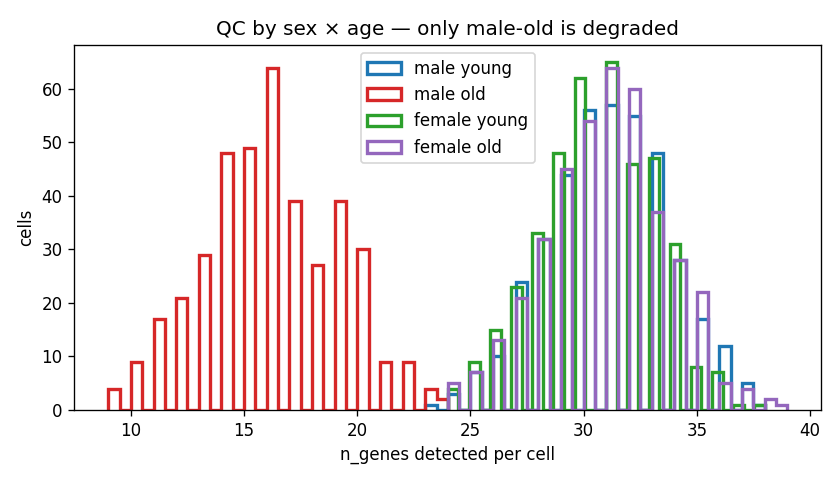
\includegraphics[width=0.78\linewidth,height=\textheight,keepaspectratio,alt={Per-cell gene detection (n\_genes) by sex and age in the synthetic worked example. Only male-old is QC-degraded (median 16 vs 31 genes), reproducing the Tabula Muris Senis interaction confound; pooling the sexes hides it.}]{figures/fig1_qc_strata.png}
\caption{Per-cell gene detection (n\_genes) by sex and age in the
synthetic worked example. Only male-old is QC-degraded (median 16 vs 31
genes), reproducing the Tabula Muris Senis interaction confound; pooling
the sexes hides it.}
\end{figure}

\textbf{GATE 0 (mathematical independence).} \texttt{mi\_3bin}'s
expectation shifts \textasciitilde61\% under simulated
\texttt{extra\_dropout} with z = 44.8 --- flagged as confounded (both
large \emph{and} reliably separated); it \emph{is} a detection metric.
Under \texttt{depth\_downsample} it shifts 22\% (z = 13.4) and under
\texttt{library\_scale} 3\% (z = 1.9), neither crossing both thresholds.
The library-normalized reference \texttt{norm\_pearson} shifts only 3\%
under dropout and 15\% under depth-downsampling --- both below the 25\%
relative-change threshold, so it passes, even though those shifts are
reliably nonzero (their separation statistics are z = 4.5 and z = 16.7,
well above \texttt{z\_thresh}). This is the key point of the AND-rule:
\texttt{norm\_pearson} does \emph{not} stay within estimator noise (a z
of 16.7 is far outside it), it stays within the \emph{effect-size}
threshold --- its expectation barely moves. That is why it passes on the
relative-change criterion, not because it is noise-free. The contrast
with \texttt{mi\_3bin} (61\% shift) shows the confound is
\emph{avoidable}, not that all metrics are doomed: the design fails the
metric whose expectation moves a lot and passes the one whose
expectation moves a little.

\textbf{GATE 2 (n\_genes matching) --- and the pooling lesson.} Run
pooled across sexes, GATE 2 \emph{passes} with the note: no meaningful
pre-matching effect (\textbar0.0044\textbar{} \textless{}
permutation-null floor 0.054) --- nothing to preserve; the groups simply
do not differ on this metric. This is the ``pooling hides the
interaction confound'' lesson made mechanical: old-female (normal)
dilutes old-male (degraded), so the pooled effect is \textasciitilde0.
Restrict to the confounded stratum --- males only --- and GATE 2 returns
\textbf{STOP}: the groups are incomparable because their n\_genes ranges
do not overlap. The confound is invisible pooled and lethal stratified.
This is the same factorial-interaction structure the real analysis
reported (ref 1), reconstructed here in synthetic form: the marginal
young-vs-old comparison is clean, the sex-by-age interaction is where
the artifact lives.

\textbf{GATE 3 (raw visibility).} The raw \texttt{Smad3} vs
\texttt{Col1a1} scatter, young vs old, shows the ``shape change'' as
points collapsing onto the zero axes --- dropout, not coupling. The gate
reports the per-group zero-fractions for you to eyeball.

\begin{figure}
\centering
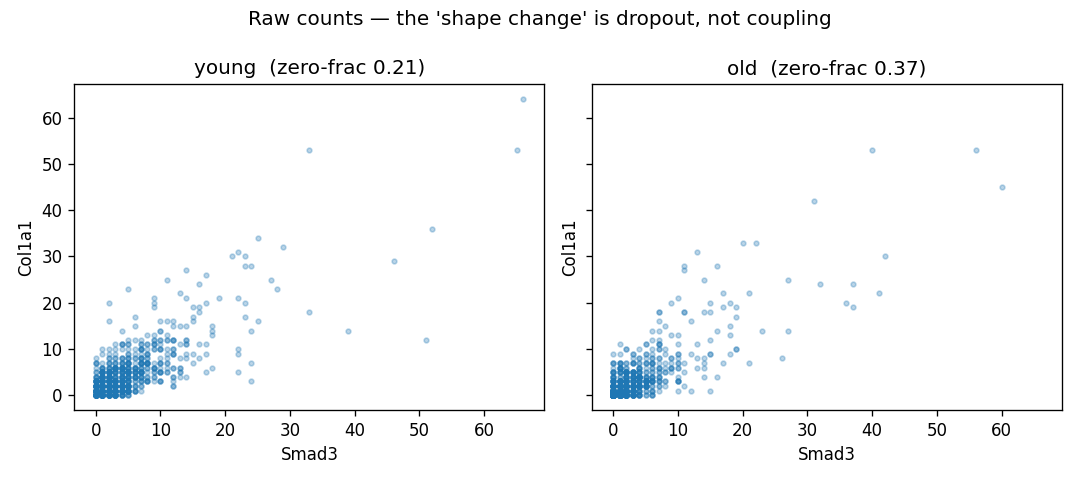
\includegraphics[width=0.88\linewidth,height=\textheight,keepaspectratio,alt={Raw Smad3 vs Col1a1 counts, young vs old. The apparent between-group shape change is dropout collapsing points onto the zero axes (zero-fraction 0.21 vs 0.37), not a change in coupling.}]{figures/fig2_raw_scatter.png}
\caption{Raw Smad3 vs Col1a1 counts, young vs old. The apparent
between-group shape change is dropout collapsing points onto the zero
axes (zero-fraction 0.21 vs 0.37), not a change in coupling.}
\end{figure}

\textbf{GATE 5 (controls).} The housekeeping pair
\texttt{Actb}-\texttt{Gapdh} fires and the random pair stays null in all
strata: PASS on this synthetic data. In the prior internal analysis (ref
1), this control was only partially reassuring --- housekeeping coupling
also declined in males once stratified --- which is why GATE 5 checks
every stratum rather than the pool.

\textbf{Verdict.} On the synthetic dataset the metric dies at GATE 0 (it
is a detection metric) and GATE 1 (the male stratum is QC-degraded), and
the confounded stratum is not even comparable at GATE 2. This matches
the \emph{by-hand} retroactive audit of the real metric recorded in ref
1 --- where the automated gates were never run --- which marked the real
metric FAIL on the first applicable gate (GATE 0) and additionally on
gates 1, 2, 3, and 6, with GATE 5 a partial fail; the judgment gates (4,
7) were not scored for MI, so ``every applicable gate that was checked
failed'' is the honest statement, not a literal ``N of N passed'' tally.
Either way the conclusion of that audit was that the real metric was not
measuring biology. What \emph{did} survive that audit and would survive
here: the sex dimorphism in cell quality itself (male-old cells detect
far fewer genes --- real, whether biological or technical), and
\texttt{Actb}-\texttt{Gapdh} co-expression, which survives n\_genes
matching in both sexes.

\begin{center}\rule{0.5\linewidth}{0.5pt}\end{center}

\section{Discussion}\label{discussion}

\textbf{Scope.} This is a workflow and tool contribution, not a
biological-results paper: the worked example is a synthetic dataset
patterned on the real phenomenon, with a documented one-line path to the
real Tabula Muris Senis and CELLxGENE skin data (the real autopsy is not
run here; see Section 3 and the closing note). The scope is deliberately
single-cell QC. The gates encode the specific ways scRNA-seq metrics
fake biology --- dropout, library size, detection-rate confounds,
factorial-interaction confounds, platform artifacts --- and they treat
the metric as a black box precisely so that focus is not diluted. A
metric from another domain can be passed in, but the perturbations the
harness knows how to apply (dropout, depth, library scaling, gene
subsampling) are single-cell perturbations.

\textbf{Scripted vs judgment gates.} Six gates run automatically from
the data (GATE 0, 1, 2, 3, 5, 6; GATE 6 only when a second dataset is
supplied); GATE 4 and GATE 7 are judgment gates that the skill
\emph{elicits} rather than scripts, because ``does this metric uniquely
correspond to the biology'' and ``is this effect size biologically
meaningful'' are not computable from data alone. GATE 3 is a hybrid: the
engine computes and exports the raw scatter and zero-fractions
automatically, but returns a JUDGMENT verdict for you to read. Making
the tool honest about this boundary --- auto where it can be, elicited
where it cannot --- is a design choice, not a limitation to paper over.
The pre-registration form the skill walks you through \emph{before} any
computation is the mechanism that enforces the ``state your commitments
first'' inversion.

On the three motivating failures, the honest attribution is: only Error
3 (MI coupling) would have been caught by a \emph{scripted} gate in 45
seconds (GATE 1 QC parity). Error 1 (ACP) needed the
cross-platform/depth evidence that GATE 0 and GATE 6 formalize but that
GATE 6 marks SKIP without a second dataset the user must supply; Error 2
(beta-heart) dies only at judgment GATE 4, which the tool elicits rather
than scripts. So the tool would have flagged all three, but two of the
three needed the judgment or replication machinery, not the fast
automatic screen.

\textbf{Self-audit.} The tool was subjected to an adversarial
\emph{code} audit --- a review of the software's correctness and
robustness, not an independent scientific review of the gates' validity
--- and 24 findings were fixed as a result. The engine ships with a
self-test suite (35/35 passing, including the adversarial-audit
regressions, a follow-up integrity pass that made GATE 6 stratify and
dropped a measured no-op perturbation, and SimpleData-vs-AnnData
agreement). The suite confirms that the \emph{implementation behaves as
specified}: on the one planted dataset it separates a known-confounded
metric (\texttt{mi\_3bin}) from a known-clean one
(\texttt{norm\_pearson}), catching the artifact without also failing the
reference metric. This is a demonstration on a single planted confound,
not a validation of the gates' sensitivity or specificity (see
Limitations); a green test suite shows the code runs as written, not
that the gates are scientifically sound. A validator that can only bless
things is useless, so \texttt{mi\_3bin} is included specifically as a
metric that \emph{should} fail.

\textbf{Limitations.} The gates are \textbf{necessary, not sufficient}.
Passing all eight does not prove a metric measures biology; it only
removes the specific artifacts these gates know about. Novel confounds
outside this list will pass silently. Beyond that, four limitations are
worth stating plainly.

\emph{The thresholds are uncalibrated heuristics.} Every pass/fail knob
--- \texttt{tol} = 0.25, \texttt{z\_thresh} = 4.0, the 1.5x QC ratio,
\texttt{overlap\_min} = 0.2, \texttt{keep\_frac} = 0.5,
\texttt{max\_frac} = 3.0, \texttt{balance\_ratio} = 1.1, the GATE 5 20\%
band, the GATE 3 dropout gap of 0.15, \texttt{min\_cells} --- is a
chosen default, not a value derived or calibrated to a target error
rate. No correction is applied for the many perturbations and factorial
strata tested across the suite, so the family-wise false-positive
behavior is uncharacterized. Users should treat the defaults as starting
points and expose the ones that matter for their metric.

\emph{The gates' own sensitivity and specificity are unquantified.} The
demonstration is a single planted confound at high severity (30\%
capture in one stratum) versus one clean reference metric on one
dataset. There is no ROC, no sweep over confound strength, no test that
the gates catch weaker confounds, and no measurement of the
false-positive rate on genuinely clean metrics across a range of data.
The self-test is an anecdote of correctness, not a validation of the
method.

\emph{The bootstrap baseline is approximate.} GATE 0 judges
perturbations against a bootstrap-resample baseline treated as estimator
noise. Bootstrap preserves the empirical distribution but changes ties
and effective sample size, and for finite-sample-biased estimators ---
plug-in mutual information in particular --- resampling with replacement
can itself perturb the estimate. The estimator-noise band GATE 0 relies
on is therefore approximate for exactly the class of metrics (MI) the
tool most often targets.

\emph{No correlation metric is fully depth-invariant under dropout.}
This is a limitation the tool cannot fix. \texttt{norm\_pearson} passes
GATE 0 on the synthetic example, but ``passes GATE 0 here'' is not
``immune to depth'' --- as its 15\% depth-downsample shift shows,
library normalization reduces the dependence, it does not abolish it.
GATE 6 in v0.1 also requires the user to supply the second dataset, and
does not enforce that it is a different platform. The right posture is
that the gates convert an unexamined red flag into an explicit, numbered
pass/fail, and that the residual is stated, not that they certify a
metric clean.

\begin{center}\rule{0.5\linewidth}{0.5pt}\end{center}

\section{Software availability}\label{software-availability}

\texttt{metric-autopsy} is distributed through two front doors backed by
one engine (\texttt{src/metric\_autopsy/}, the single source of truth):

\begin{itemize}
\tightlist
\item
  \textbf{Claude Code skill.} Drop the repository into your skills
  directory; the \texttt{metric-autopsy} skill (\texttt{SKILL.md})
  elicits a pre-registration, then runs the gates.
  Progressive-disclosure references (\texttt{references/gates.md},
  \texttt{references/red\_flags.md},
  \texttt{references/prereg\_template.md}) load on demand.
\item
  \textbf{pip package.} \texttt{pip\ install\ metric-autopsy} exposes
  the \texttt{metric-autopsy} CLI (including
  \texttt{metric-autopsy\ -\/-demo}, which runs the reference
  \texttt{mi\_3bin} failure end-to-end) and the \texttt{run\_autopsy}
  Python API. You bring a \texttt{metric(data)\ -\textgreater{}\ float}
  callable and your factorial \texttt{obs} column names.
\end{itemize}

License: \textbf{MIT}. Repository:
\href{https://github.com/mool32/metric-autopsy}{github.com/mool32/metric-autopsy}.
Archived on Zenodo --- concept-DOI
\href{https://doi.org/10.5281/zenodo.21195679}{10.5281/zenodo.21195679}
(all versions), v0.1.0
\href{https://doi.org/10.5281/zenodo.21195680}{10.5281/zenodo.21195680}.
Citation metadata: \texttt{CITATION.cff}. Reproducibility: the package
targets Python 3.9+ with only \texttt{numpy} and \texttt{pandas} as
required runtime dependencies --- \texttt{scipy} (exact KS test),
\texttt{anndata} (\texttt{.h5ad} I/O), and \texttt{matplotlib} (GATE 3
PNGs) are optional extras with pure-numpy fallbacks;
\texttt{pip\ install\ metric-autopsy} followed by
\texttt{metric-autopsy\ -\/-demo} reproduces the synthetic numbers in
Section 3 with no downloads.

\textbf{Competing interests.} The author is affiliated with Vaika Inc.;
the tool is released under a permissive open-source license and Vaika
has no commercial interest in it. \textbf{Funding.} None.

\section{Data availability}\label{data-availability}

The engine and its tests require \textbf{no external data} --- they run
on a synthetic planted confound
(\texttt{metric\_autopsy.cli.demo\_data},
\texttt{metric-autopsy\ -\/-demo}). The worked example uses only public
data, re-fetchable via
\texttt{examples/mi\_coupling\_tms/download\_data.py}:

\begin{itemize}
\tightlist
\item
  \textbf{Tabula Muris Senis} (FACS / SmartSeq2), from figshare /
  CELLxGENE Census \texttt{tabula-muris-senis}.
\item
  \textbf{Human skin fibroblasts} (10x), from CELLxGENE
  (\texttt{cellxgene.cziscience.com}, skin, 179 donors).
\end{itemize}

No inputs are irreplaceable; all are public and re-downloadable. The
genes used by the worked example are \texttt{Smad3}, \texttt{Col1a1}
(the coupling pair under test), \texttt{Actb}, \texttt{Gapdh}
(housekeeping / positive control), and an expression-matched random pair
(negative control), with factor columns \texttt{age}, \texttt{sex}, and
where available \texttt{tissue}, \texttt{cell\_type}.

\begin{center}\rule{0.5\linewidth}{0.5pt}\end{center}

\section{References and notes}\label{references-and-notes}

\textbf{External references} --- single-cell QC, batch effects, and
false-discovery methods this work builds on.

\begin{itemize}
\tightlist
\item
  Lun ATL, Bach K, Marioni JC (2016). Pooling across cells to normalize
  single-cell RNA sequencing data with many zero counts. \emph{Genome
  Biology} 17:75. doi:10.1186/s13059-016-0947-7
\item
  McCarthy DJ, Campbell KR, Lun ATL, Wills QF (2017). Scater:
  pre-processing, quality control, normalization and visualization of
  single-cell RNA-seq data in R. \emph{Bioinformatics} 33:1179--1186.
  doi:10.1093/bioinformatics/btw777
\item
  Hippen AA, Falco MM, Weber LM, et al.~(2021). miQC: an adaptive
  probabilistic framework for quality control of single-cell
  RNA-sequencing data. \emph{PLOS Computational Biology} 17:e1009290.
  doi:10.1371/journal.pcbi.1009290
\item
  Leek JT, Scharpf RB, Corrada Bravo H, et al.~(2010). Tackling the
  widespread and critical impact of batch effects in high-throughput
  data. \emph{Nature Reviews Genetics} 11:733--739. doi:10.1038/nrg2825
\item
  Luecken MD, Büttner M, Chaichoompu K, et al.~(2022). Benchmarking
  atlas-level data integration in single-cell genomics. \emph{Nature
  Methods} 19:41--50. doi:10.1038/s41592-021-01336-8
\item
  Squair JW, Gautier M, Kathe C, et al.~(2021). Confronting false
  discoveries in single-cell differential expression. \emph{Nature
  Communications} 12:5692. doi:10.1038/s41467-021-25960-2
\item
  Neufeld A, Gao LL, Popp J, Battle A, Witten D (2024). Inference after
  latent variable estimation for single-cell RNA sequencing data.
  \emph{Biostatistics} 25:270--287. doi:10.1093/biostatistics/kxac047
\item
  Lähnemann D, Köster J, Szczurek E, et al.~(2020). Eleven grand
  challenges in single-cell data science. \emph{Genome Biology} 21:31.
  doi:10.1186/s13059-020-1926-6
\end{itemize}

\textbf{Internal notes and data.}

\begin{enumerate}
\def\labelenumi{\arabic{enumi}.}
\tightlist
\item
  \textbf{Origin document.} \emph{Metric validation checklist: lessons
  from ACP, beta-heart, and MI coupling} (2026), an unpublished internal
  write-up (a self-report, not an independently validated result) that
  recorded the three failures with their numbers and first articulated
  the gate system, including the by-hand retroactive audit of the real
  MI metric. All real numbers in Sections 1 and 3 (male young/old 3670
  vs 1540 = 2.4x; ACP rho = -0.54 on SmartSeq2, -0.09 on 10x, +0.38 at
  500 genes; beta 12-lead AUC = 0.98 LBBB vs RBBB) are drawn from it and
  are not re-derived in this manuscript.
\item
  \textbf{Software reference.} \texttt{metric-autopsy} v0.1.0,
  \texttt{references/gates.md} (prose gate rationale for the skill) and
  \texttt{references/red\_flags.md}. These follow the implementation in
  \texttt{src/metric\_autopsy/}; in particular GATE 0 perturbs the
  user's own data (a bootstrap baseline plus dropout/depth/library
  perturbations of the observed matrix), not a separately synthesized
  null dataset.
\item
  \textbf{Worked example.}
  \texttt{examples/mi\_coupling\_tms/notebook.ipynb}. All numbers in
  Section 3 (male-stratum 1.94x n\_genes ratio, 0.00 overlap;
  \texttt{mi\_3bin} dropout shift \textasciitilde61\%, z = 44.8, depth
  22\%, z = 13.4; \texttt{norm\_pearson} dropout shift 3\%, z = 4.5,
  depth 15\%, z = 16.7; pooled effect \textasciitilde0 below null floor
  0.054; males STOP on non-overlapping ranges) are from the
  \textbf{synthetic} dataset and are labeled as such throughout.
\item
  \textbf{Data sources.} Tabula Muris Senis (figshare / CELLxGENE
  Census); human skin, CELLxGENE (cellxgene.cziscience.com). See
  \texttt{DATASETS.md}.
\end{enumerate}

\emph{Note on honesty of claims: this preprint reports a tool and a
synthetic worked example with a documented path to real data. It does
not report real-data autopsy results; the automated gates have not been
run on the real data. The real-data outcomes cited in Sections 1 and 3
are drawn from the by-hand retroactive audit in ref 1, an unpublished
internal self-report, and are attributed as such rather than presented
as results of this work.}

\end{document}
